\documentclass{article}
\usepackage{riju,multicol,subcaption,hyperref}
\hypersetup{colorlinks,linkcolor=blue,citecolor=blue}
\usepackage[margin=0.5in]{geometry}
\title{\textsc{A Study in Scotchlet}}
\author{\textsc{Abhigyan (Riju) Dasgupta}}
\date{\textsc{June 27, 2016}}

\renewenvironment{abstract}
 {\small
  \begin{center}
  \bfseries \abstractname\vspace{-.5em}\vspace{0pt}
  \end{center}
  \list{}{
    \setlength{\leftmargin}{3cm}%
    \setlength{\rightmargin}{\leftmargin}%
  }%
  \item\relax}
 {\endlist}

 \renewcommand\refname{\large References}
 \newlength{\figwig}
 \newlength{\figsig}
 \setlength{\figwig}{0.42\paperwidth}
 \setlength{\figsig}{0.43\paperwidth}

\begin{document}
\maketitle
\begin{abstract}
2427 days (nearly seven years) of personal alcoholic beverage consumption data are categorized and visualized. Drinks are classified by type, quantity, and date. A first analysis of frequency distributions and cumulative ethanol consumption curves is performed, and an attempt is made to develop predictive quantitative models, without conclusive results.
\end{abstract}

\begin{multicols}{2}
\raggedcolumns
	\subsection*{Introduction}
	On November 7, 2009, I ingested an alcoholic beverage for the first time. In an effort to gain deeper understanding of my life choices, I began keeping a record of every drop of alcohol I ever drank, by date, quantity, and beverage name. At the time, I believed my alcohol consumption would be sufficiently low that this would prove to be a trivial task, but the record of alcoholic beverages consumed has since grown into a large text-based dataset. Recent developments have made it feasible to analyze these data using tools previously out of my reach. This paper will present my findings, observe patterns and trends, and attempt to develop predictive models for future alcohol consumption.

	\subsection*{Data and Methods}
	\subsubsection*{Raw Data}
	We first examine the format and content of the available raw data. The data are a simple human-readable list of dates, with each date followed by a list of names of beverages, accompanied by the number of standard US drinks of that beverage consumed. A standard drink is a beverage containing about 14 grams of pure ethanol, or about 0.6 fl oz (17.7 mL). Standard drink equivalents are typically summarized as one of the following \cite{nih}:
	\begin{itemize}
		\setlength\itemsep{0.05em}
		\item 12 oz of beer (5\% ABV)
		\item 5 oz of wine (12\% ABV)
		\item 1.5 oz of liquor (40\% ABV)
	\end{itemize}
	As can be easily verified, given the percent ABV and total volume, each of these drink archetypes contain one standard drink. Thus, by recording the number of standard drinks, as opposed to the volume of the beverage, the data are more easily legible, as well as more normalized with respect to other entries. Not only is it often unfeasible (as well as unnecessary) to record the volume of the beverage, as alcohol consumption often takes place ``in the wild'' without access to volumetric flasks, recording standard drinks also circumvents the laborious procedure of post-consumption web searches to determine the ABV of each beverage so as to convert the beverage volume into the actual parameter of interest: the volume of pure ethanol. Moreover, standard drink units are more intuitive than milliliters or fluid ounces on a human scale, and thus make it simpler to look over anomalies and patterns ``by eye.'' Nevertheless, by choosing to implicitly convert each drink into standard drink units at the time of data taking, I introduced a large source of error into the data almost immediately upon its creation.
	
	\vspace*{-.5em}
	\subsubsection*{Sanitization and Categorization}
	With this raw dataset I undertook the sanitization and categorization of the data. First, any anomalies (including sporadic records of beverage volume in fl oz or mL, instead of standard drink units) were corrected. Fractions were converted to decimals, and superfluous punctuation, comments, and annotation were removed.
	
	Second, I took the decision to standardize the keyword ``sip'' as 0.1 standard drinks. Sips are a poorly defined quantity ranging from a few drops to half a mouthful, but without any further information, I am forced to standardize a quantitative definition of ``sip''.
	
	Third, every drink was classified as either beer, wine, or liquor. In the vast majority of cases the beverage name, my memory, and/or additional information were sufficient to disambiguate the type of drink. A few entries required performing a web search for the drink name, with varying degrees of success. A small handful were not unambiguously categorized; for these, I made an educated guess. For this classification, the alcohol content as well as the \emph{social role} of the drink were taken into account; as such, cocktails, weak liquors such as Malibu and Baileys, and Four Loko were classified as liquor, while drinks such as Smirnoff Ice, Mike's Hard, and Seagram's Escapes were classified as beer. This is because the former play the \emph{role} of liquor in social settings, while the latter play the \emph{role} of beer in social settings. Finally, champagne was of course classified as wine.

	Following this process, the cleaned dataset's entries consist of dates, with a beer, wine, or liquor label for each drink, as well as a decimal number describing the quantity of the drink in US standard drink units.
	
	For more details on the possible uncertainties due to the effects of using standard drink units, standardizing sips to 0.1 standard drinks, or the manual classification of drinks by type, see the section on Error Analysis.
	\subsection*{Analysis}
	\subsubsection*{Global Statistics}
	We are now in a position to perform some elementary numerical analysis on the data. Of the 2427 days from November 7, 2009 to June 30, 2016, I consumed at least one sip of an alcoholic beverage on 494 of them, or 20\%. I have consumed 29~L (8~gal) of pure ethanol in my lifetime, of which 12~L (42\%) was from beer, 10~L (35\%) was from liquor, and 7~L (23\%) was from wine. Figure~1 visualizes this breakdown.
	\begin{center}
		Figure 1: Ethanol consumption by type.
		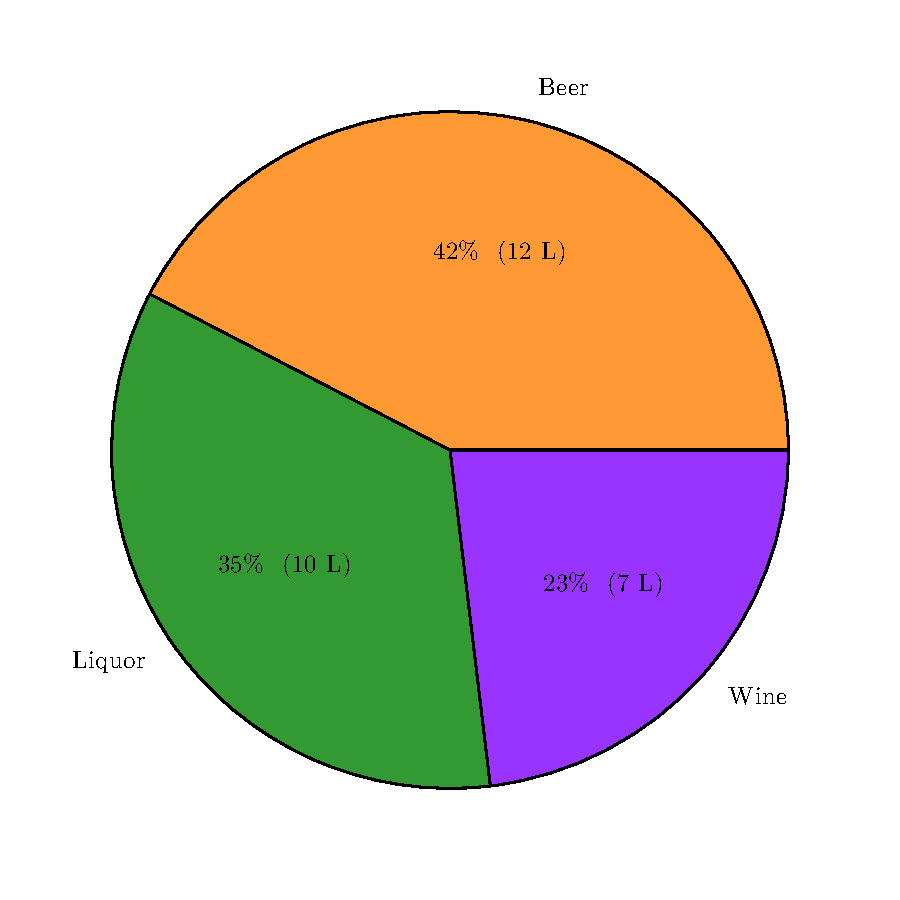
\includegraphics[width=0.7\columnwidth]{pie.pdf}
	\end{center}
	\setcounter{figure}{1}
	
	I drank beer before liquor on 76 days, which is 67\% of the days I drank both beer and liquor. It is uncertain whether on those days I had never been sicker, although it can be stated with some confidence that of the 4 days in my life that overconsumption of alcohol has led to vomiting, only on one of them did I drink beer before liquor. A sample size of 4, however, is far too low to come to any reasonable conclusions, and the investigation of the adage is left for further study.
	
	\subsubsection*{Over Time}

	\begin{figure*}[htb]
		\centering
		\begin{subfigure}[b]{\figsig}
			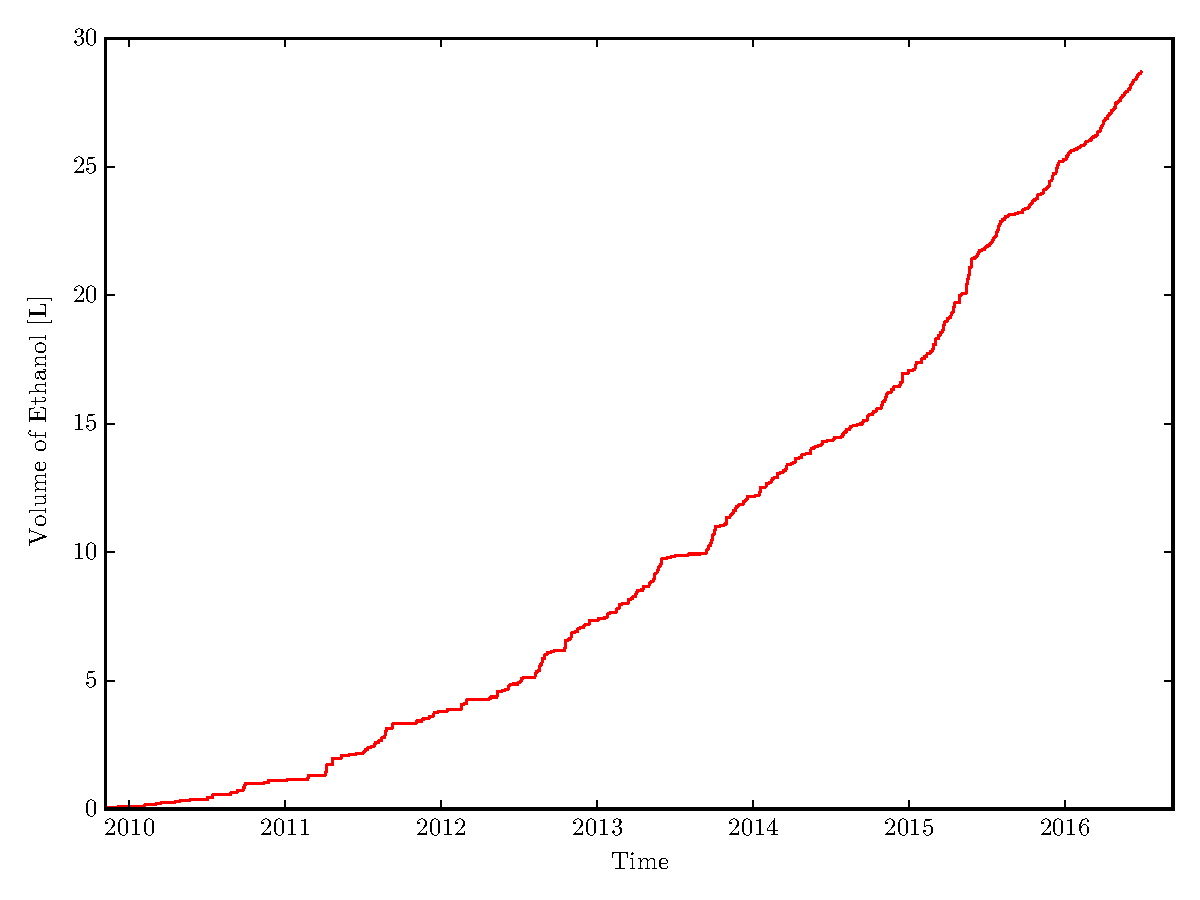
\includegraphics[width=\textwidth]{time.pdf}
			\caption{Total}
			\label{time-total}
		\end{subfigure}
		\begin{subfigure}[b]{\figsig}
			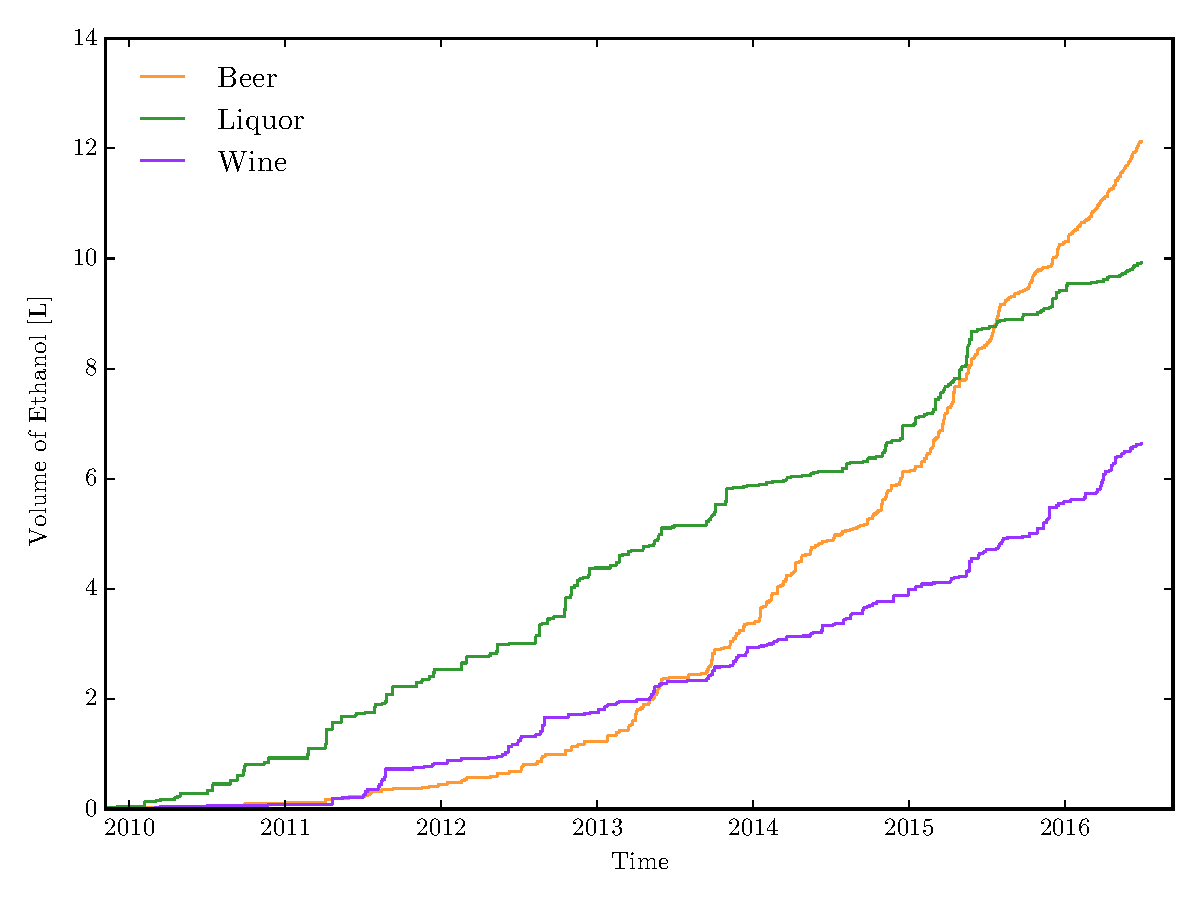
\includegraphics[width=\textwidth]{time-alc.pdf}
			\caption{By type}
			\label{time-alc}
		\end{subfigure}
		\caption{Cumulative lifetime ethanol consumption vs. time.}
	\end{figure*}

	The first and most obvious plot of interest is alcohol consumption vs. time. Figures~\ref{time-total} and \ref{time-alc} show cumulative lifetime ethanol consumption over time, both overall and by time. It is interesting to associate trends on these plots with life events. For example, the rise in wine consumption in the summer of 2011 corresponds to the summer during which I studied abroad in Cambridge, UK, where the alcohol consumption was both legal (for a 19 year old) and culturally distinct, i.e. wine and beer were consumed more frequently and casually, but less acutely, and liquor consumption rarely reached ``binge drinking'' levels, defined as 5 or more drinks in 2 hours \cite{cdc}.

	Other relevant events include turning 21 during the third quarter of 2012, corresponding approximately to when my tastes shifted from early-college liquor consumption to a more restrained savoring of beer and wine; the summer of 2013, during which I was at home and consumed very little alcohol; the beginning of graduate school during the third quarter of 2013, correlated with an increase in social beer consumption; a slight reduction in rate in the summer of 2014, during which I was studying for my comprehensive exams; and the summer of 2015, when I moved to Europe, where the drinking culture is distinct; see preceding paragraph.
	
	\subsubsection*{Frequency Distributions}
	\begin{figure*}[!p]
		\centering
		\begin{subfigure}[b]{\figwig}
			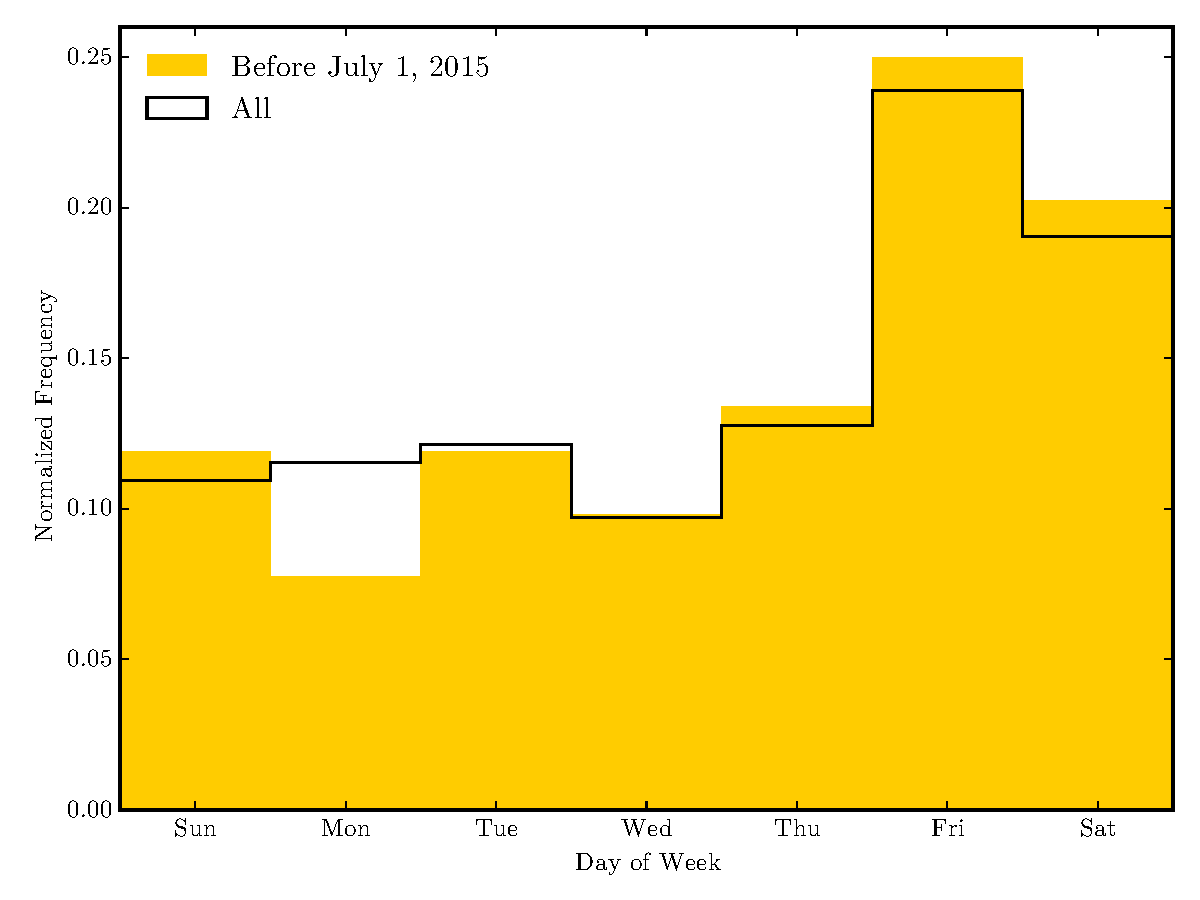
\includegraphics[width=\textwidth]{wd.pdf}
			\caption{Number of days, normalized}
			\label{wd}
		\end{subfigure}
		\begin{subfigure}[b]{\figwig}
			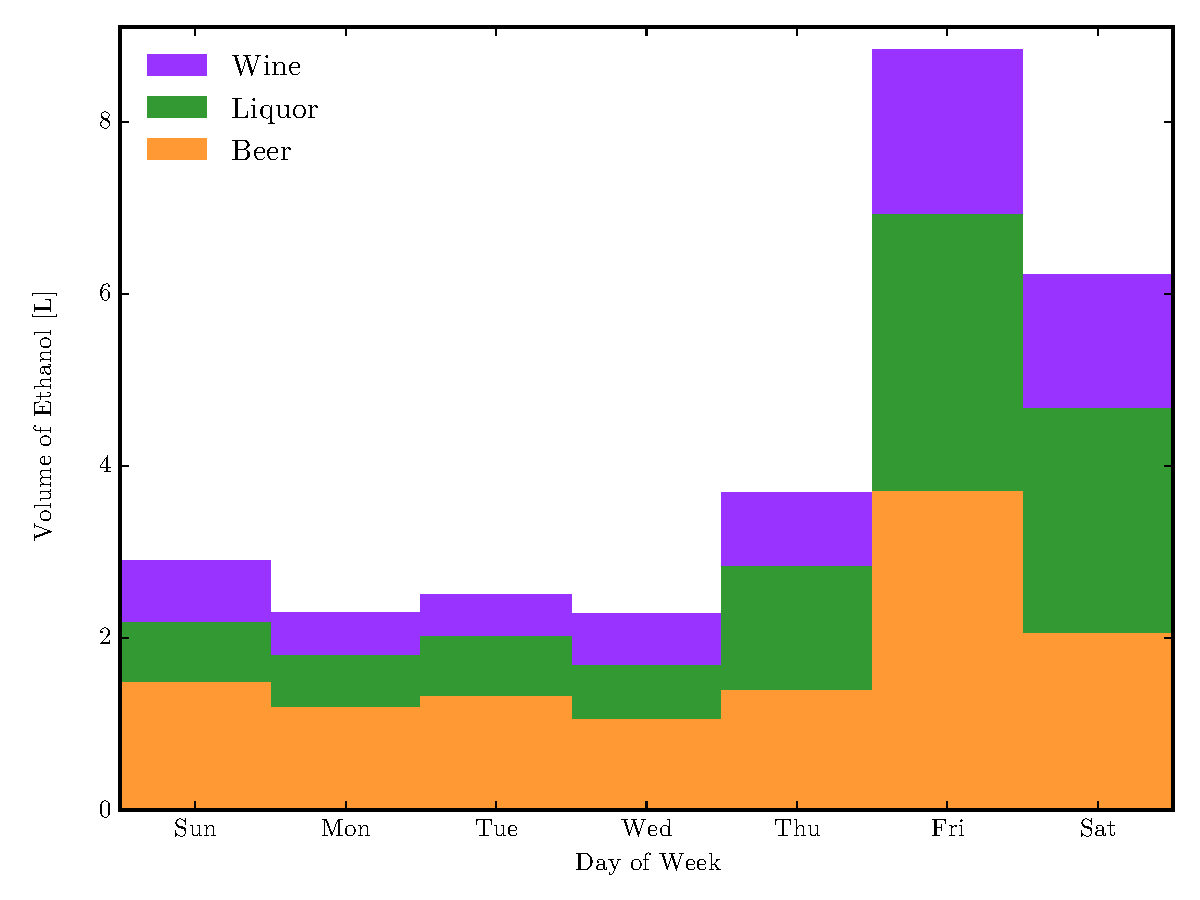
\includegraphics[width=\textwidth]{wd-alc.pdf}
			\caption{By type}
			\label{wd-alc}
		\end{subfigure}
		\caption{Frequency distributions parameterized by weekday.}
	\end{figure*}
	Figure~\ref{wd} shows the normalized frequency distribution of drinking days as a function of the day of week, while Figure~\ref{wd-alc} shows the same frequency distribution weighted by the drink type. As one might expect, the distribution shows a peak on Fridays, followed by Saturdays, while the middle of the week shows significantly less alcohol consumption.
	
	An interesting effect was observed. Upon first inspection of all the data (the black line in Figure~\ref{wd}), I noticed that the event count for Mondays was higher than one might expect, comparable to Sundays. However, restricting the data and selecting only the events prior to July 1, 2015 yields the orange distribution, which is closer to a ``stereotypical'' frequency distribution. The excess in Monday drinking can be explained by the fact that Mr. Pickwick's Pub Quiz in Geneva is on Monday evenings, and I started attending this pub quiz when I moved to Europe in early July. It is surprising that one year of pub quizzes could affect the distribution in a single bin by 5\%. A closer look at the distribution without any preselection, but weighted by volume of ethanol in Figure~\ref{wd}, reveals that the frequency distribution by number of days is artificially inflated and does not necessarily correspond to significantly more drinking on Mondays. That is, while the number of Mondays on which alcohol was consumed is comparatively high with respect to the other days of the week, the actual volume of ethanol consumed is not.

	\begin{figure*}[!p]
		\centering
		\begin{subfigure}[b]{\figwig}
			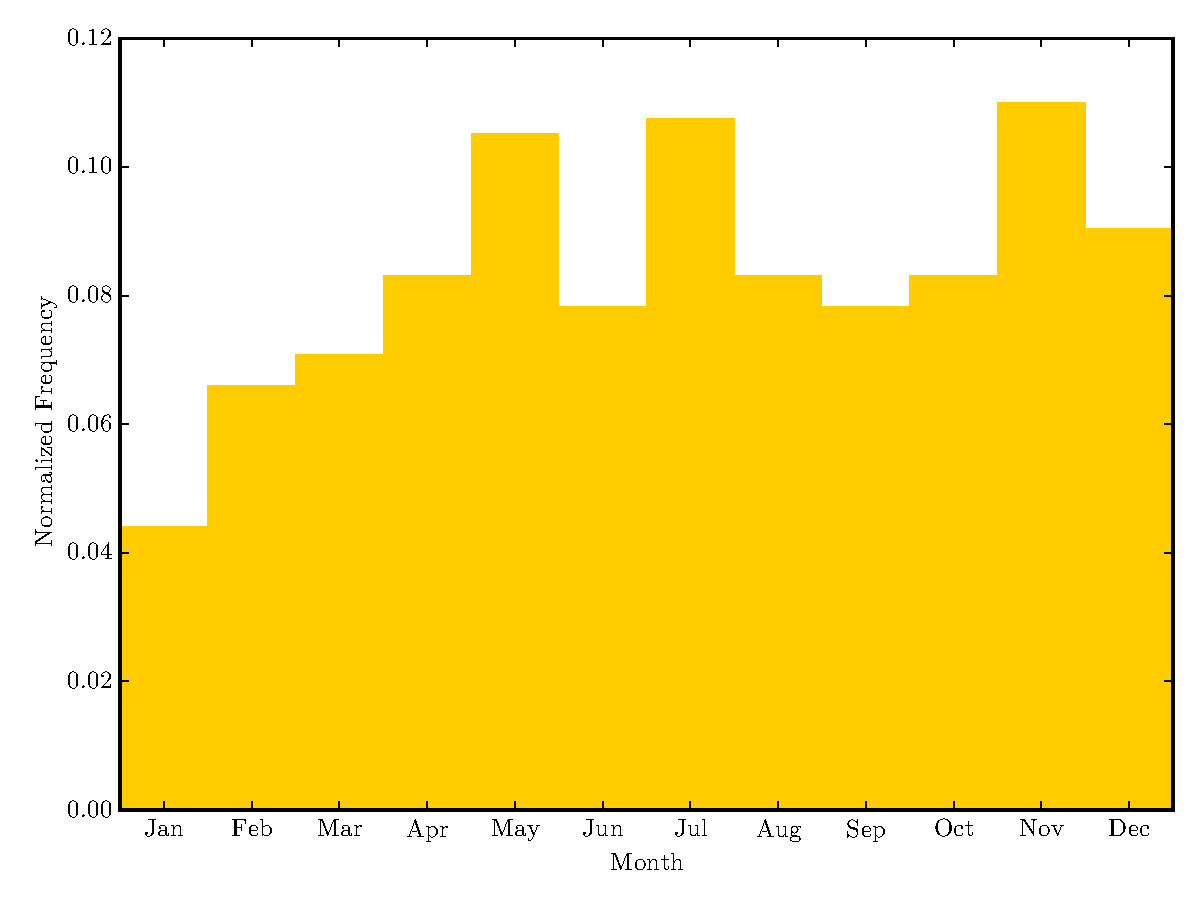
\includegraphics[width=\textwidth]{mo.pdf}
			\caption{Number of days, normalized}
			\label{mo}
		\end{subfigure}
		\begin{subfigure}[b]{\figwig}
			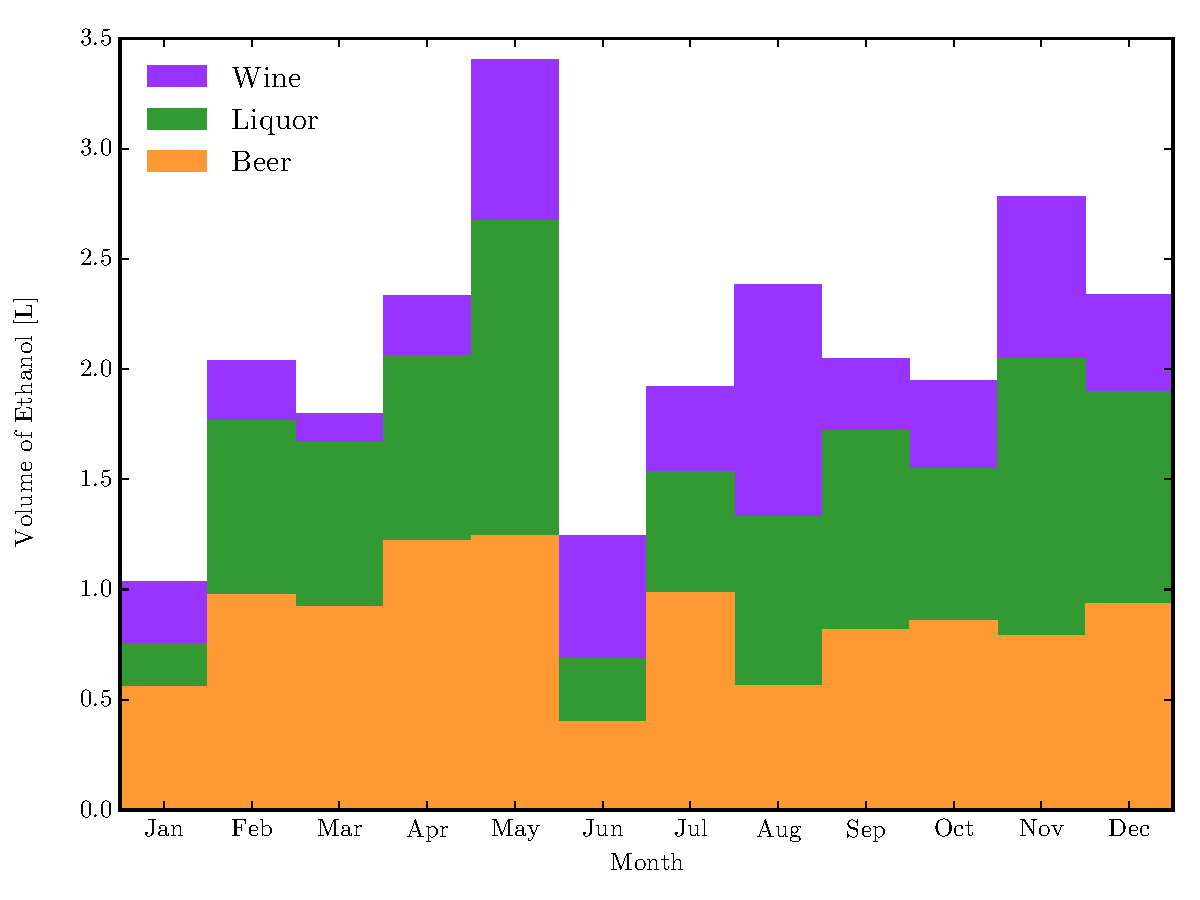
\includegraphics[width=\textwidth]{mo-alc.pdf}
			\caption{By type}
			\label{mo-alc}
		\end{subfigure}
		\caption{Frequency distributions parameterized by month, through December 2015.}
	\end{figure*}

	Figure~\ref{mo} shows the normalized frequency distribution of drinking days as a function of the month, while Figure~\ref{mo-alc} shows the same frequency distribution weighted by the drink type. To prevent skewing the data due to only half of 2016 having elapsed, only data prior to 2016 are included in these histograms. Alcohol consumption is lowest during January and June, months I have previously spent mostly at home (although this is likely to change as I spend years in Europe) and increases steadily towards the end of the academic year, likely due to end-of-year cheer and festivities. There are also peaks in late summer (a summer month I am typically not at home) and November (a month containing Thanksgiving and the aftermath of my birthday).

	\begin{figure*}[!p]
		\centering
		\begin{subfigure}[b]{\figwig}
			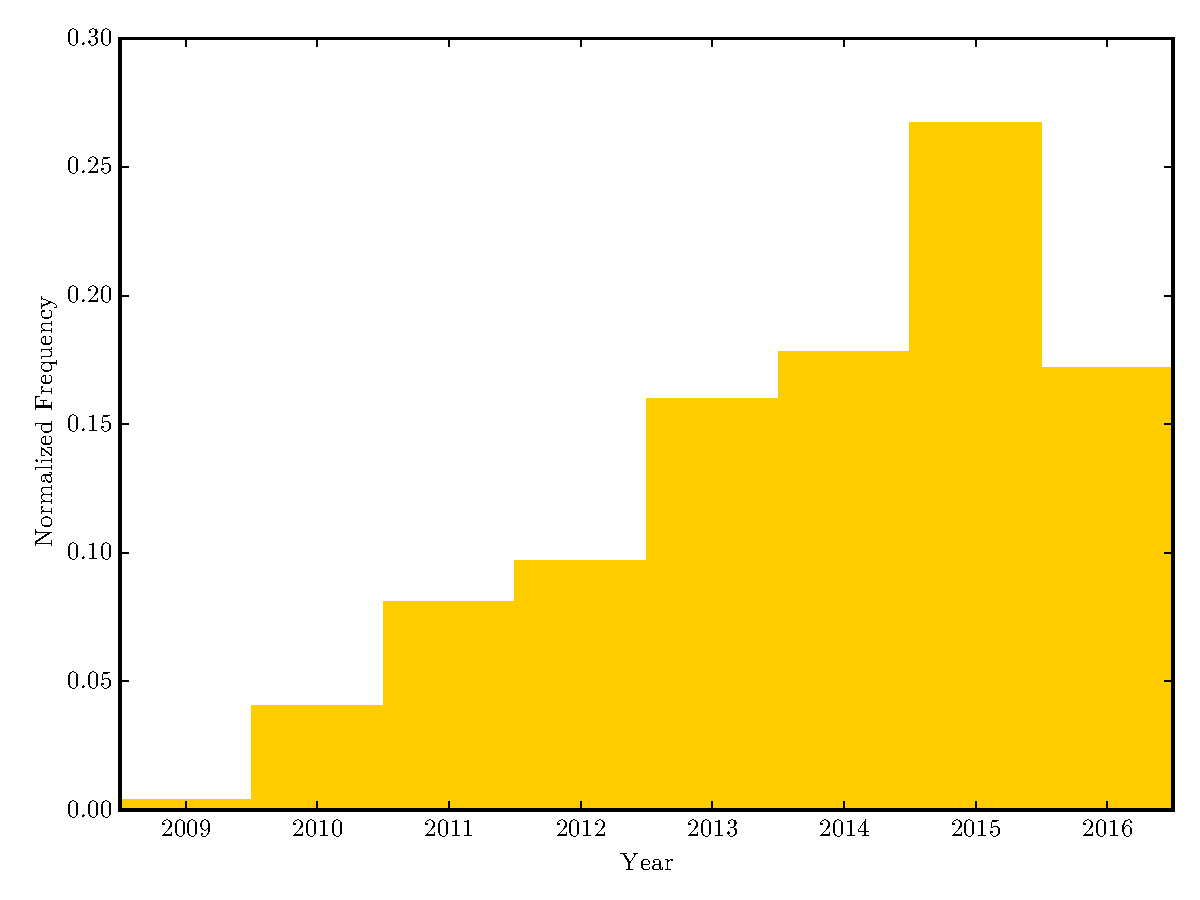
\includegraphics[width=\textwidth]{yr.pdf}
			\caption{Number of days, normalized}
			\label{yr}
		\end{subfigure}
		\begin{subfigure}[b]{\figwig}
			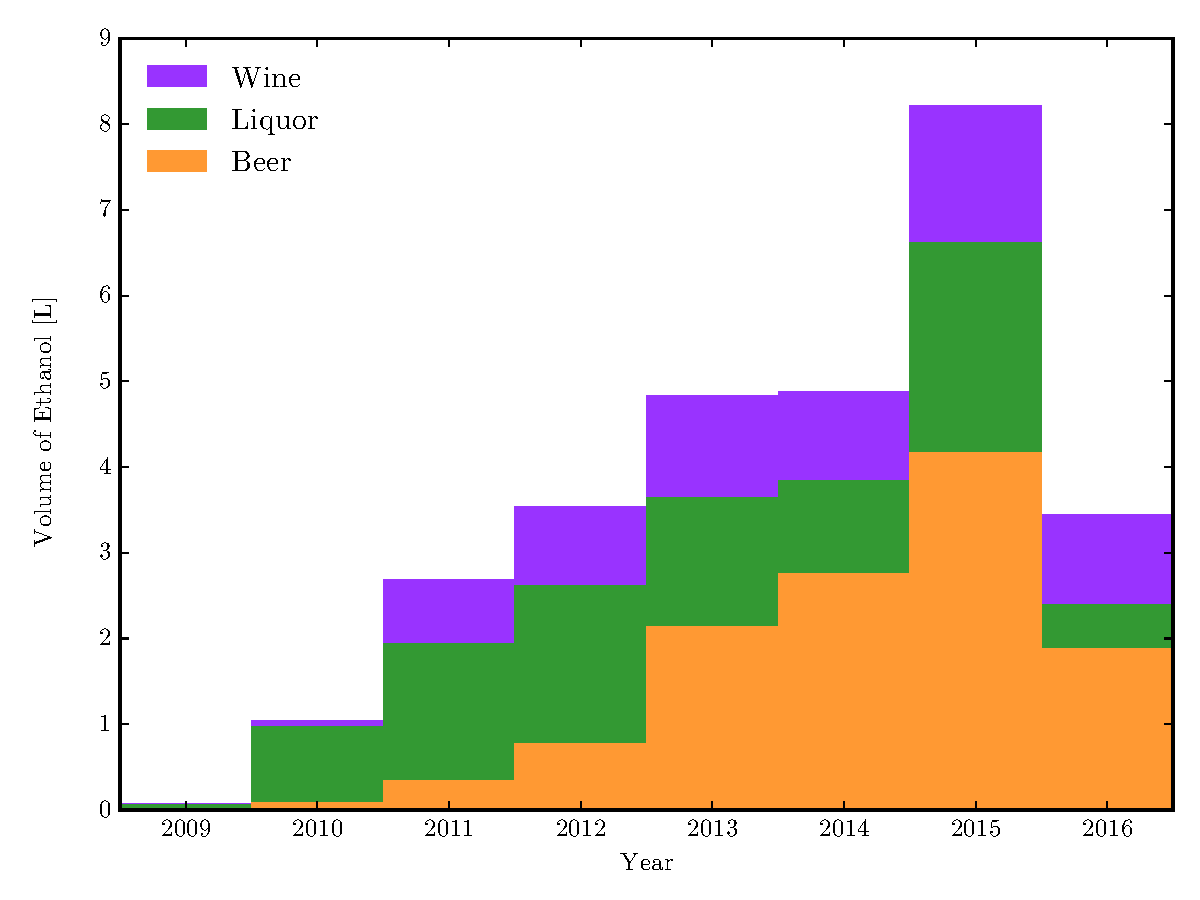
\includegraphics[width=\textwidth]{yr-alc.pdf}
			\caption{By type}
			\label{yr-alc}
		\end{subfigure}
		\caption{Frequency distributions parameterized by year.}
	\end{figure*}

	Figure~\ref{yr} shows the normalized frequency distribution of drinking days as a function of the year, while Figure~\ref{yr-alc} shows the same frequency distribution weighted by the drink type. Obviously, alcohol consumption for 2016 is low due to only half of 2016 having elapsed. The frequency distribution by month through 2015 suggests that I drink 47\% of my annual ethanol by the end of June. Assuming the same density distribution in 2016 (i.e.\ I have already consumed 47\% of my annual alcohol this year) leads to a prediction of
	$$V_{2016}^\text{th} = V_{2016}^\text{obs}\frac{V_\text{global}^\text{Jan-Dec}}{V_\text{global}^\text{Jan-Jun}} = 7.4\text{ L}$$
	This is a projected 10\% decrease in annual ethanol consumption. Figure~\ref{mo-pre} shows Figure~\ref{mo-alc}, i.e.\ the distribution by month through 2015, normalized to 1, and superimposed with the distribution in 2016 so far, normalized to 0.47. Figure~\ref{mo-pre} shows that the distribution in 2016 may differ significantly compared to previous years, so the aforementioned projected decrease may be too optimistic.
	
	\begin{figure*}[htbp]
		\centering
		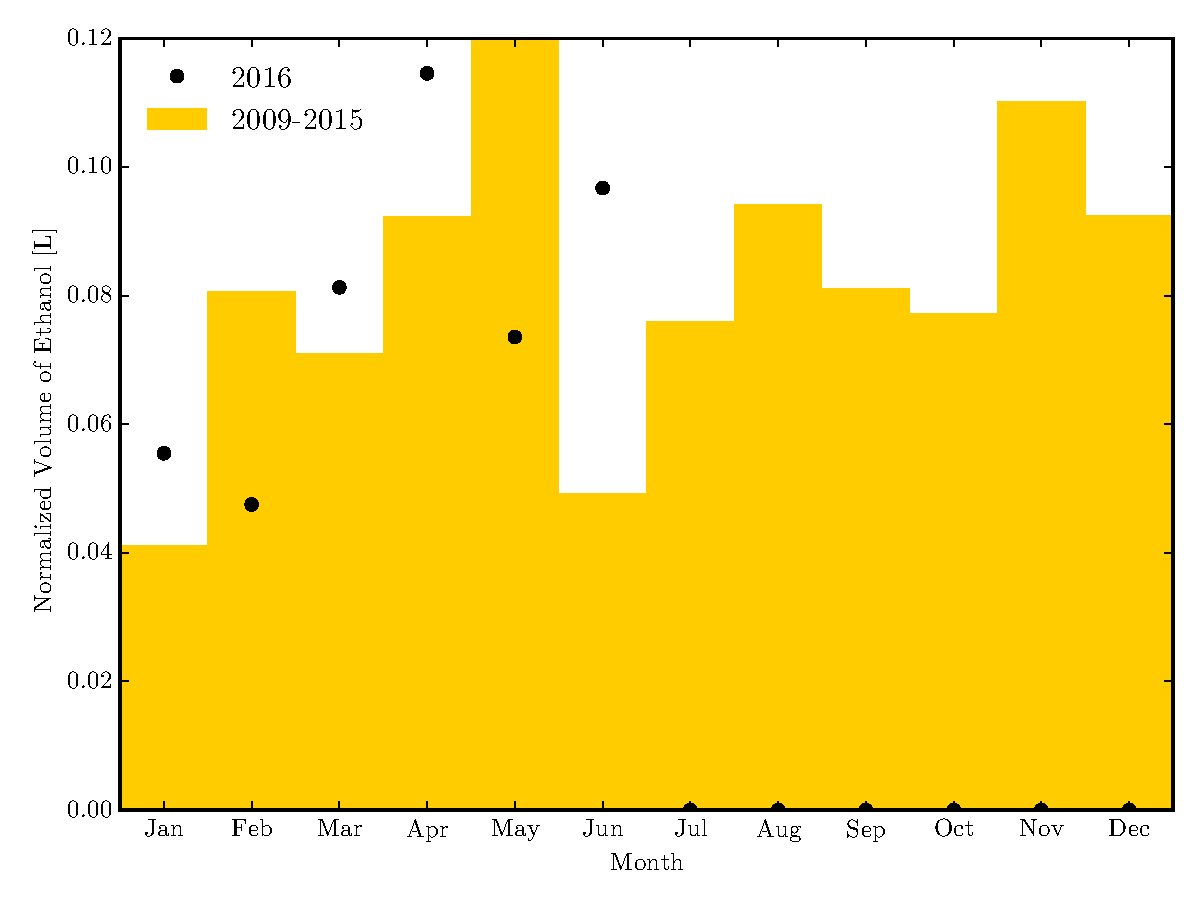
\includegraphics[width=0.6\paperwidth]{mo-pre.pdf}
		\caption{Normalized ethanol volume consumed by month, with 2016 data scaled to 47\%.}
		\label{mo-pre}
	\end{figure*}

	While the steep increase in alcohol consumption during 2015 may look alarming at first glance, it should be noted that my ethanol consumption for 2015 (8.2~L) is still less than the WHO projected per capita ethanol consumption in liters for 2015 for the United States (9.0~L), and is comparable to the regional average (8.1~L) \cite{who}. Furthermore, cause for concern diminishes further given that my place of residence is now Europe, where the regional average is 10.2~L per capita, and the consumption per capita for France and Switzerland are 11.6~L and 10.6~L, respectively \cite{who}. Cause for alarm is justified, however, if one extrapolates the rising trend in alcohol consumption to 2016, which would indicate an annual ethanol consumption rivaling that of the entire world with the possible exception of Belarus, or if one considers the global average, 6.3~L per capita. It is uncertain whether or not I am destined for liver disease, and this topic is left for further study.

	\subsubsection*{Binge* Drinking}
	Another quantity of interest is the time between drinks. The time resolution is of course one day, so an appropriate distribution would be the number of consecutive dry days, i.e.\ the number of consecutive days without a single drink. Figure~\ref{intertime} shows this distribution. On a log scale, the distribution seems to exhibit linearity, motivating a test for consistency with an exponential distribution. First, a linear least-squares regression was performed and overlaid, as the dashed line. The Pearson product-moment correlation coefficient \cite{lyons-cc} between the log of the frequency and the time between drinks is 
	$$\rho = -0.9314$$
	A strong correlation is found between these quantities. However, caution is required, as this correlation is not evidence of consistency with an exponential distribution. The standard metric for distribution testing is the chi-squared goodness-of-fit test. Our situation requires some thought before the application of the test, so we first describe the standard procedure \cite{lyons-chi}. As this is a histogram, the frequencies are traditionally expected to be Poisson distributed with a mean and variance equal to the frequency (i.e.\ the error on a bin with $N$ events is $\sqrt{N}$). The observed values are $y_i^\text{obs}$, the theoretical values (from the fit) are $y_i^\text{th}$, and the errors are $\sigma_i = \sqrt{y_i}$. The chi-squared test statistic is computed as
	$$\chi^2 = \sum_{i=1}^n{\frac{\left(y_i^\text{obs} - y_i^\text{th}\right)^2}{\sigma_i^2}}$$
	The test statistic is then compared to a $\chi^2$ distribution with $n-3$ degrees of freedom (nominally $n-1$, minus 2 for the two-parameter fit). From this, a $p$-value may be computed (from the cumulative distribution function, or the integral of the $\chi^2$ distribution:
	$$p = 1 - \int_0^{\chi^2}{\chi^2_{n-3}}$$
	Now, our situation differs from the standard situation somewhat. The fit was an unweighted, least-squares linear regression applied to the \emph{log} of the frequencies. Thus, the values of $y_i^\text{obs}$ are not raw counts, as is required. Additionally, the logarithm biases the fit in favor of lower observed frequencies. Finally, the errors are not simply the square root of the observed values, because the observed values are the log of the frequencies. Attempting to handle these issues in a straightforward manner is beyond the scope of this paper, so instead, we will apply the chi-squared test to several situations, modifying the quantity used as $y_i^\text{obs}$, the errors used in computing the $\chi^2$, the weights used in the fitting process, and the type of fitting process used. Table~\ref{types} summarizes the situations.

	\begin{table*}
		\centering
		\begin{tabular}{ccccc}
				& $y_i^\text{obs}$ & $\sigma_i$ & $w_i$ & Process \\
			1 & $N_i$        & $\sqrt{N_i}$ & $1/N_i$ & Non-linear
		\end{tabular}
		\caption{Summary of fitting situations}
		\label{types}
	\end{table*}


	Another quantity of interest is the distribution of the number of drinks in a single day. Figure~\ref{dpd} shows this distribution. Unsurprisingly, the number of drinks in a day decreases in frequency with the number of drinks. These quantities exhibit an exponential relationship, as shown by the linear fit in Figure~\ref{dpd}.

	\begin{figure*}[htbp]
		\centering
		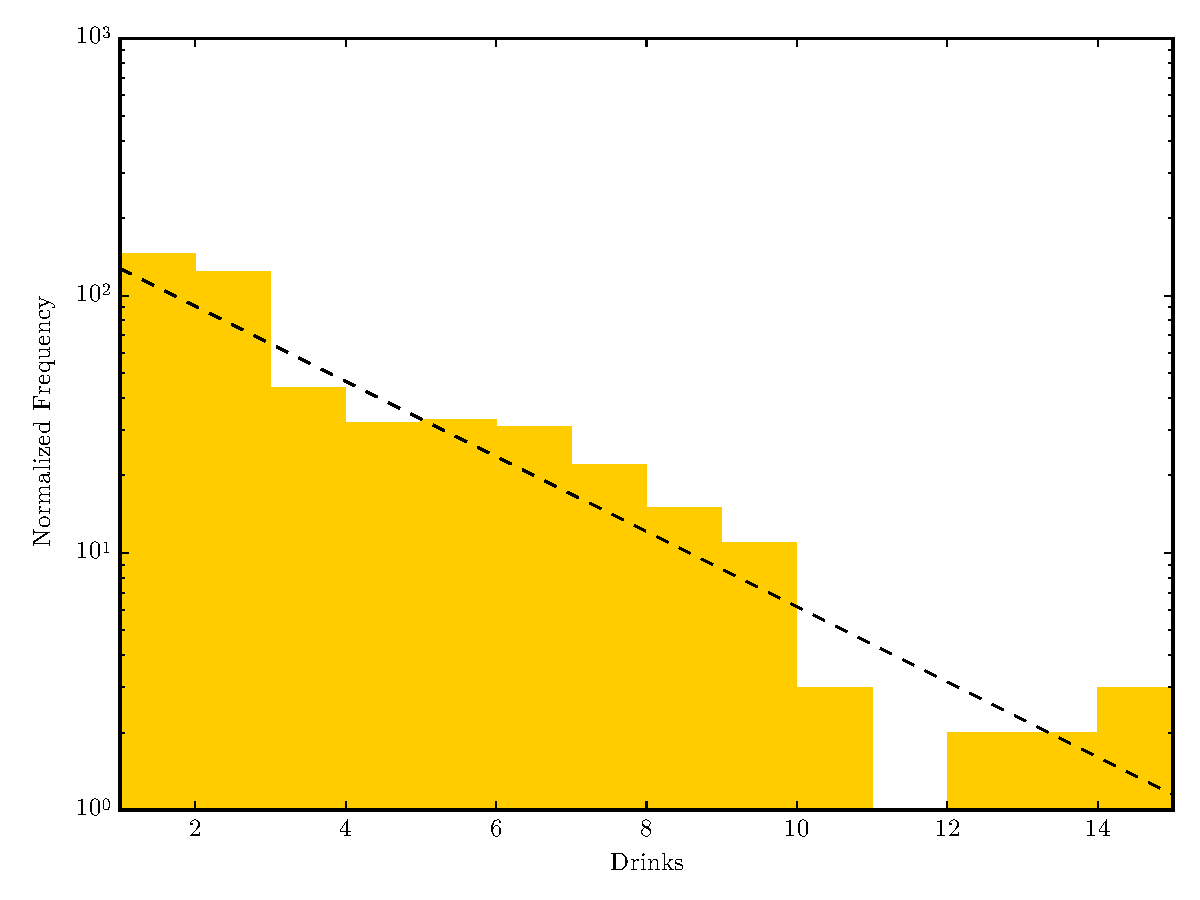
\includegraphics[width=0.6\paperwidth]{dpd.pdf}
		\caption{Normalized frequency of drinks in a single day, log scale}
		\label{dpd}
	\end{figure*}

	\subsection*{Conclusion}
	\begin{thebibliography}{9}
		\bibitem{nih}
			NIAAA, NIH. \emph{``What is a Standard Drink?''} \url{http://pubs.niaaa.nih.gov/publications/Practitioner/pocketguide/pocket_guide2.htm}. Retrieved June 27, 2016.
		\bibitem{cdc}
			CDC. \emph{``Fact Sheets - Binge Drinking.''} \url{http://www.cdc.gov/alcohol/fact-sheets/binge-drinking.htm}. Retrieved June 27, 2016.
		\bibitem{who}
			WHO. \emph{Alcohol per capita consumption.} \url{http://apps.who.int/gho/data/node.sdg.3-5-viz?lang=en}. Retrieved June 27, 2016.
		\bibitem{lyons-cc}
			Lyons, Louis. \emph{Statistics for nuclear and particle physicists.} Cambridge University Press, 1986, Section 3.4, pp. 59--60.
		\bibitem{lyons-chi}
			Lyons, Louis. \emph{Statistics for nuclear and particle physicists.} Cambridge University Press, 1986, Sections 4.5--4.6, pp. 105--115.
	\end{thebibliography}
\end{multicols}

\end{document}
